\documentclass{beamer}
\usetheme{metropolis}
\usepackage{graphicx}
\usepackage{subfig}
\title{Safe Return Doubtful: Week 7}
\date{\today}
\author{Jordan Hanson}
\institute{Whittier College Department of Physics and Astronomy}

\begin{document}
\maketitle

\section{Summary}

\begin{frame}{Summary}
\begin{enumerate}
\item Biological research in Antarctica
\begin{itemize}
\item Big creatures: photo essay
\item Orcas
\item Undersea alien worlds
\end{itemize}
\item SCINI and Deep-SCINI: Submersible Capable of Under Ice Navigation and Imaging
\end{enumerate}
\end{frame}

\section{Big Creatures}

\begin{frame}{Big Creatures}
TED-talk by world-reknowned photographer: \\ \vspace{1cm}
\url{https://www.ted.com/talks/paul_nicklen_tales_of_ice_bound_wonderlands?utm_campaign=tedspread&utm_medium=referral&utm_source=tedcomshare}
\end{frame}

\section{Orca Hunting Technique}

\begin{frame}{Orcas}
The following is a quote from this week's reading, chapter 21 about Ponting, the photographer upon the \textbf{Terra Nova} landing. \\ \vspace{0.5cm}
\textit{they thought he was a seal and getting right under the floe bumped so hard they split off one piece with him on and it was only by the greatest agility he escaped ... what irony of fate to be eaten by a whale thinking one was a seal and then spat out because one was only a photographer.} \\ \vspace{0.5cm}
Example of this behavior: \url{https://youtu.be/g1VEwsI4SlY}
\end{frame}

\section{Undersea Alien Worlds}

\begin{frame}{Undersea Alien Worlds}
Several interesting features of life under ice shelves and sea ice:
\begin{enumerate}
\item Where is the food? \textit{Benthic community}
\item Where is the light?  How does photosynthesis take place?
\item How do we explore these areas?
\end{enumerate}
\textbf{Science Under the Ice}: Explorer's Cove
\url{https://youtu.be/L6EsroRPZ4c} \\ \vspace{0.5cm}
\end{frame}

\section{SCINI and Deep-SCINI}

\begin{frame}{SCINI and Deep-SCINI}
SCINI: Submersible Capable of Under Ice Navigation and Imaging
\begin{figure}
\centering
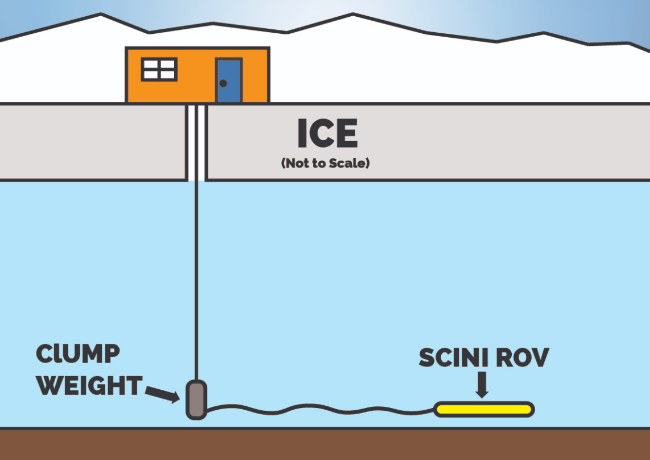
\includegraphics[width=0.6\textwidth]{scini.png}
\caption{\label{fig:scini} Part of the SCINI system is held down with the clump weight (left) and the cables and power flow through to the ROV at right.}
\end{figure}
\end{frame}

\begin{frame}{SCINI and Deep-SCINI}
What about a syntactic-foam encrusted ROV with sapphire windows on its cameras?
\begin{itemize}
\item Withstands enormous pressures
\item Can take photos and videos
\item Soil samples
\begin{enumerate}
\item Benthic communities often thrive on detritis in soil
\item Soil samples reveal no significant nutrients in the soil, though
\end{enumerate}
\end{itemize}
\textbf{SCINI and Deep-SCINI}: ROVs
\url{https://youtu.be/vnVdR8goVXg}
\end{frame}

\section{Summary}

\begin{frame}{Summary}
\begin{enumerate}
\item Biological research in Antarctica
\begin{itemize}
\item Big creatures: photo essay
\item Orcas
\item Undersea alien worlds
\end{itemize}
\item SCINI and Deep-SCINI: Submersible Capable of Under Ice Navigation and Imaging
\end{enumerate}
\end{frame}

\end{document}